
\documentclass[slovak, 11pt]{beamer}
\usepackage[slovak]{babel}
\usepackage[utf8]{inputenc}
\hypersetup{unicode=true}

\usepackage{graphicx}
\usepackage[export]{adjustbox}  %adjust pics

\usepackage{blindtext}          %for independent footnote
\newcommand\blfootnote[1]{\begingroup\renewcommand\thefootnote{}\footnote{#1}\addtocounter{footnote}{-1}\endgroup}

\usetheme{AnnArbor}             %theme
\usecolortheme{beaver}          %color of the theme

\setbeamertemplate{items}[square]                           %square items
\setbeamercolor{item}{fg=black}                             %black items
\setbeamertemplate{section in toc}[square]                  %square items in intro
\setbeamercolor{block title}{bg=black!90,fg=yellow}         %yellow-black classic block
\setbeamercolor{alerted text}{bg=yellow!85!orange,fg=red}   %red-yellow alert box
\setbeamercolor{example text}{bg=red!70!black,fg=white}
\setbeamercolor{bibliography entry author}{fg=red!70!black} % red bibliography

%%%%%%%%%%%%%%%%%%%%%%%%%%%%%%%%%%%%

\title{Typografie a~publikování\,--\,5.~projekt}
\subtitle{Lineárny zoznam}
\author{Natália Bubáková}
\institute{VUT FIT}
\date{\today}

%%%%%%%%%%%%%%%%%%%%%%%%%%%%%%%%%%%

\begin{document}

\begin{frame}
  \titlepage
\end{frame}

%%%%%%%%%%%%%%%%%%%%%%%%%%%%%%%%%%%

\begin{frame}{Prehľad}
  \tableofcontents
\end{frame}

%%%%%%%%%%%%%%%%%%%%%%%%%%%%%%%%%%%

\section{Dátové štruktúry}

\begin{frame}{Dátové štruktúry}
    \textbf{Dátová štruktúra} je \dots
    \begin{itemize}
        \item logická reprezentácia dát, poradie jej prvkov a~vzťahy medzi nimi
        \item spôsob uloženia jej prvkov a~toho ako s~nimi možno pracovať
        \item môže byť \emph{lineárna} alebo \emph{nelineárna}
    \end{itemize}
    
    \begin{minipage}{0.46\textwidth}
    \begin{block}{Typy dátových štruktúr:}
        \begin{itemize}
            \item pole (\emph{array})
            \item front (\emph{queue})
            \item slovník (\emph{dictionary})
            \item zásobník (\emph{stack})
            \item halda (\emph{heap})
            \item strom (\emph{tree})
            \item bunka s využitím smerníka
        \end{itemize}
    \end{block}
    \end{minipage}
    \hspace{0.5cm}
    \begin{minipage}{0.46\textwidth}
    \begin{block}{}
        \begin{itemize}
            \item dátum a čas
            \item množina (\emph{set})
            \item trieda (\emph{class})
            \item vektor (\emph{vector})
            \item graf
            \item zobrazenie (\emph{map})
            \item zoznam (\emph{list})
            \item \textbf{spájaný zoznam} (\emph{linked list})
        \end{itemize}
    \end{block}
    \end{minipage}
\end{frame}


%%%%%%%%%%%%%%%%%%%%%%%%%%%%%%%%%%%%%%

\section{Úvod do lineárneho zoznamu}

\begin{frame}{Prečo práve \emph{lineárny zoznam} ?}
    Medzi najčastejšie využívané dátové štruktúry patrí \emph{pole}
    \begin{block}{Pole (array)}
        \begin{itemize}
            \item[$+$] je ľahké na pochopenie
            \item[$+$] jednoduchý prístup k~jednotlivým prvkom 
        \end{itemize}
        \emph{ale} \dots
        \begin{itemize}
            \item[$-$] ukladá sa len do súvislej pamäti (\emph{contiguous memory})
            \item[$-$] má pevne určenú dimenziu
            \item[$-$] raz po uvedení jeho veľkosti je táto nemenná
            \item[$-$] vloženie a~zmazanie jeho prvkov je veľmi pracné
        \end{itemize}
    \end{block}
    \dots a~práve tieto obmedzenia pokrýva lineárny zoznam (\emph{linked list})
\end{frame}

%%%%%%%%%%%%%%%%%%%%%%%%%%%%%%%%%%%%

\begin{frame}{A čo to je ten \emph{lineárny zoznam} !?}
    \begin{block}{Lineárny\,/\,spájaný zoznam (\emph{linked list})}
        \begin{itemize}
            \item je lineárna štruktúra, ktorá pozostáva zo sekvencie prvkov, zvaných \emph{uzle}
            \item každý prvok pozostáva z~dvoch častí
            \begin{enumerate}
                \item obsah uložených dát v~danom prvku
                \item odkaz (adresa) na nasledujúci prvok
            \end{enumerate}
        \end{itemize}
        \begin{figure}[h]
          \vspace{-40pt}
          
\includegraphics[width=4.5cm,right]{linked_list_1.png} 
        \end{figure}
    \end{block}
    \begin{exampleblock}{Príklad:}
        Jednodúchý lineárny zoznam čísiel 10, 20, 30 sa dá zobraziť ako:
        \begin{figure}[h]
          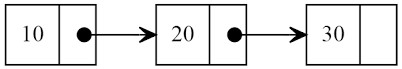
\includegraphics[width=6.5cm,center]{linked_list_2.jpg} 
        \end{figure}
    \end{exampleblock}
\end{frame}

%%%%%%%%%%%%%%%%%%%%%%%%%%%%%%%%%%%

\section{Typy lineárných zoznamov}

\begin{frame}{Typy lineárných zoznamov}
    \begin{block}{Jednosmerný lineárny zoznam (\emph{singly linked list})}
        \begin{itemize}
            \item je sekvencia uzlov pozostávajúcich z~dát a~jedného ukazovateľa na nasledujúci uzol, tzv. \emph{next} \hfill $\square \rightarrow \square \rightarrow \square \rightarrow \dots$
        \end{itemize}
    \end{block}
    \begin{block}{Obojsmerný lineárny zoznam (\emph{doubly linked list})}
        \begin{itemize}
            \item je sekvencia uzlov pozostávajúcich z~dát a~dvoch ukazovateľaov na predošlý a~nasledujúci uzol, tzv. \emph{next} a \emph{previous} \hfill $\square \rightleftarrows \square \rightleftarrows \square \rightleftarrows \dots$
        \end{itemize}
    \end{block}
    \begin{block}{Cyklický lineárny zoznam (\emph{circular linked list})}
        \begin{itemize}
            \item je sekvencia uzlov, kde posledný uzol drží ukazovateľ na prvý uzol, a~tak tvorí uzavretý \uv{logický kruh} \hfill $\rightarrow \square \rightarrow \square \rightarrow \dots \rightarrow \square \rightarrow$
        \end{itemize}
    \end{block}
    \blfootnote{Jednosmerný lineárny zoznam predstavuje základ pre všetky spomenuté, preto sa pre účeľ tejto prezentácie ďalej venujeme práve tomuto typu.}
\end{frame}

%%%%%%%%%%%%%%%%%%%%%%%%%%%%%%%%

\section{Štruktúra}

\begin{frame}{Štruktúra}
    \begin{figure}[h]
      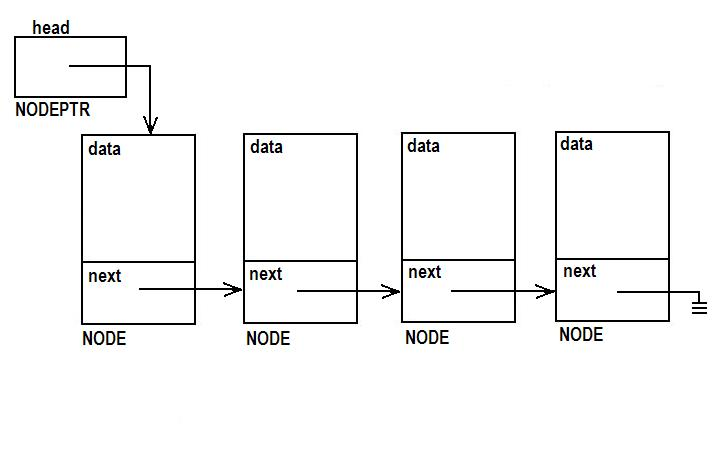
\includegraphics[width=9cm,center]{linked_list_3.jpg} 
      \vspace{-4.5em}
    \end{figure}
    \begin{alertblock}{Sekvencia prvkov}
        pozostáva nie len z~uzlov so samotnými dátami, ale tiež 
        \begin{itemize}
            \item z~referenčného ukazovateľa na začiatok zoznamu, tzv. \emph{head} 
            \item z~posledného uzla, tzv. \emph{tail} ukazujúc na koniec, teda \emph{NULL}
        \end{itemize}
    \end{alertblock}
\end{frame}

%%%%%%%%%%%%%%%%%%%%%%%%%%%%%%%%

\begin{frame}[fragile]{Náhľad na kód}
    \begin{minipage}{0.50\textwidth}
    \begin{exampleblock}{Zostavenie zoznamu (z 3 uzlov):}

\begin{verbatim}
int main(){
 struct Node* head   = NULL;
 struct Node* second = NULL;
 struct Node* third  = NULL;\end{verbatim}
 
    \end{exampleblock}
    \end{minipage}
    \hspace{0.5cm}
    \begin{minipage}{0.35\textwidth}
    \begin{block}{Štruktúra uzla:}
    
\begin{verbatim}
struct Node{
  int data;
  struct Node *next;
};\end{verbatim}

    \end{block}
    \end{minipage}
    \begin{exampleblock}{}
    
\begin{verbatim}
 head   = (struct Node*)malloc(sizeof(structNode));
 second = (struct Node*)malloc(sizeof(struct Node));
 third  = (struct Node*)malloc(sizeof(struct Node));\end{verbatim}
 
    \end{exampleblock}
    \begin{exampleblock}{}

\begin{verbatim}
head   -> data = 1;          head   -> next = second;
second -> data = 2;          second -> next = third;
third  -> data = 3;          third  -> next = NULL;
return 0;
}\end{verbatim}

    \end{exampleblock}
\end{frame}

%%%%%%%%%%%%%%%%%%%%%%%%%%%%%%%

\section{Praktické využitie}

\begin{frame}[fragile]{Praktické využitie}
    \begin{exampleblock}{Vloženie nového uzlu (\emph{insertion})}
        \verb|void push(struct Node** head_ref, int new_data){| \\
        \begin{enumerate}
            \item {\color{red!70!black}alokovať priestor pre nový uzol}\\
            {\footnotesize\verb|struct Node* new_node = (struct Node*) malloc(sizeof(struct Node));|}
            \item {\color{red!70!black}vložiť dáta do nového uzlu}\\
            \verb|new_node->data = new_data;|
            \item {\color{red!70!black}ukazateľom ho pripojiť na zoznam}\\
            \verb|new_node->next = (*head_ref);|
            \item {\color{red!70!black}uistiť sa, že \emph{head} ukazuje na začiatok}\\
            \verb|(*head_ref) = new_node;|\\
            \verb|}|
        \end{enumerate}
    \end{exampleblock}
\end{frame}

%%%%%%%%%%%%%%%%%%%%%%%%%%%%%%%%%%

\begin{frame}[fragile]{}
\small
    \begin{exampleblock}{Vymazanie existujúceho uzlu (\emph{deletion})}
        \verb|void deleteNode(struct Node** head_ref, int key){|
        \begin{enumerate}
            \item {\color{red!70!black}vytvoriť si pomocnú premennú zo začiatku zoznamu}\\
            \verb|struct Node *temp = *head_ref, *prev;|
            \item {\color{red!70!black}skontrolovať či nie je hľadaný klúč v~prvom prvku}\\
            {\footnotesize\verb|if (temp != NULL && temp->data == key)|
            \verb|{*head_ref = temp->next; free(temp);return;}|}
            \item {\color{red!70!black}nájsť daný prvok podľa klúču}\\
            {\footnotesize\verb|while (temp != NULL && temp->data != key)|
            \verb|{prev = temp;temp = temp->next;}|}
            \item {\color{red!70!black}overiť si či sa prvok nachádza v~zozname}\\
            \verb|if (temp == NULL) return;|
            \item {\color{red!70!black}presunúť ukazovateľ tak, aby preskočil nežiadaný prvok}\\
            \verb|prev->next = temp->next;|
            \item {\color{red!70!black}uvoľniť alokovanú pamäť}\\
            \verb|free(temp); }|
        \end{enumerate}
    \end{exampleblock}
\end{frame}

%%%%%%%%%%%%%%%%%%%%%%%%%%

\section{Zhrnutie}

\begin{frame}{Zhrnutie}
    \begin{block}{Výhody}
        \begin{itemize}
            \item[$+$] Lineárny zoznam je v~pamäti dynamicky alokovaný, teda netreba vopred vedieť jeho veľkosť a~možno ho kedykoľvek pohodlne rožšíriť.
            \item[$+$] Vloženie a~vymazanie uzlu sa da jednoducho zrealizovať.
            \item[$+$] Vhodné na implementáciu fronty, grafu či zásobníku.
            \item[$+$] Jeho štruktúra výrazne znižuje prístupový čas.
        \end{itemize}
    \end{block}
    \begin{block}{Nevýhody}
        \begin{itemize}
            \item[$-$] Ukazovateĺe zaberajú navyše priestor v~pamäti.
            \item[$-$] K~prvkom sa nedá pristupovať náhodne, treba senkvenčne prejsť každým jedným uzlom.
        \end{itemize}
    \end{block}
\end{frame}

%%%%%%%%%%%%%%%%%%%%%%%%%%%

\begin{frame}{Použité zdroje}
    \begin{block}{}
    	\begin{thebibliography}{10}
    		\bibitem{} Wikipédia: Údajová štruktúra
    		\newblock \href{https://sk.wikipedia.org\%C3\%9Adajov\%C3\%A1_\%C5\%A1trukt\%C3\%BAra}{https://sk.wikipedia.org/wiki}
    		
    		\bibitem{} Study tonight: Introduction to linked list
    		\newblock \href{https://www.studytonight.com/data-structures/introduction-to-linked-list}{https://www.studytonight.com}
    		
    		\bibitem{} Slide Share: Linked list in data structure
    		\newblock \href{https://www.slideshare.net/shameen23/linked-list-in-data-structure}{https://www.slideshare.net}
    		
    		\bibitem{} Geeks for geeks: Linked List Data Structure
    		\newblock \href{https://www.geeksforgeeks.org/data-structures/linked-list/}{	https://www.geeksforgeeks.org}
    	\end{thebibliography}
    \end{block}
\end{frame}

\end{document}
